\documentclass[12pt,letterpaper,final]{article}
\usepackage[left=2cm,rigth=1.5cm,top=1.5cm,bottom=1.5cm]{geometry}
\usepackage[utf8]{inputenc}
\usepackage{amsmath}
\usepackage{amsfonts}
\usepackage{amssymb}
\usepackage{graphicx}
\usepackage{kpfonts}
\usepackage{tabularx}
\usepackage{hyperref}
\usepackage{natbib}
\usepackage{colortbl}
\usepackage{tikz}
\usepackage{ragged2e} % Paquete para justificar el texto

\title{Estimación de la posición relativa al estacionamiento de un vehículo mediante cámaras y sensores para parqueo automático en simulación}
\author{Rubén Martínez González}
%\tutor{Dr. Arturo Espinosa Romero}
\date{Marzo 2024}

\begin{document}

    \maketitle
    \begin{center}
        Asesor: Dr. Arturo Espinosa Romero

    \end{center}
    \clearpage

    \section*{Introducción}
    \noindent
    El avance continuo en la tecnología de vehículos autónomos representa un logro significativo en la revolución del transporte.
    Existe la necesidad de desarrollar sistemas ``inteligentes'' que permitan a estos vehículos aprender a conducir de manera autónoma y,
    al mismo tiempo, detectar posibles colisiones y reaccionar de manera similar a como lo haría un conductor humano.
    La convergencia de la inteligencia artificial, la visión computacional y los sistemas de control ha generado una nueva era en la movilidad,
    desafiando y redefiniendo las fronteras de la conducción convencional.
    Si bien los avances en la conducción autónoma han sido significativos, la detección y respuesta a
    situaciones de peligro, como colisiones inminentes, siguen siendo un desafío complejo.\\ \newline
    En este contexto, este trabajo se centra en el desarrollo de un sistema de detección y evasión de colisiones basado en visión computacional.
    Para lograr este desarrollo se conformará un entorno simulado que refleje el escenario de conducción de un vehículo,
    y mediante algoritmos de visión computacional se analizará la información proveniente de cámaras y sensores.
    Con el procesamiento de estos datos se podrá modelar el medio que rodea al vehículo, lo que posibilitará
    el desarrollo de estrategias de detección y evasión de colisiones en diferentes situaciones de manejo.
    Una vez que se ha realizado el procesamiento exhaustivo de los datos provenientes de cámaras y sensores mediante técnicas de visión computacional,
    se plantea la posibilidad de emplear algoritmos de aprendizaje por refuerzo.
    Los algoritmos de aprendizaje por refuerzo, al recibir estos datos procesados como entrada, tienen la capacidad de aprender de manera progresiva
    a tomar decisiones inteligentes en tiempo real.
    Aprovechando la retroalimentación proporcionada por el entorno, estos algoritmos pueden mejorar continuamente su capacidad para reaccionar y evitar colisiones.\\ \newline
    La seguridad en la carretera y la confianza del público en esta tecnología dependen en gran medida de la capacidad
    de los vehículos autónomos para enfrentar situaciones de tráfico de manera eficiente y segura.
    Esta investigación busca abordar esta problemática crítica, avanzando hacia el escenario en el que los vehículos autónomos
    sean capaces de igualar e incluso superar las habilidades de conducción humana en términos de detección y respuesta
    a situaciones de colisión.
    \clearpage

    \section*{Contexto y problemática}
    \noindent
%    problemas en los estacionamientos
    Los estacionamientos son imprescindibles en la via urbana, ya que permiten a los conductores estacionar sus vehículos
    de manera segura y eficiente. Sin embargo, el proceso de estacionamiento puede ser complicado y estresante,
    especialmente en áreas congestionadas con espacio limitado y visibilidad reducida.
    Factores como la falta de espacio, la presencia de obstáculos y la poca visibilidad para el conductor ocasionan
    dificultades al estacionar un vehículo, lo que puede aumentar el riesgo de colisiones y daños al vehículo.
    \\
%   se han logrado sistemas de asistencia al conductor
    En la actualidad, la búsqueda de soluciones para mejorar la eficiencia y seguridad en el desplazamiento vehicular
    ha llevado al desarrollo de sistemas avanzados de asistencia al conductor.
    Entre estos sistemas, el estacionamiento automático ha ganado relevancia como una función que puede contribuir
    a reducir los riesgos asociados con el estacionamiento en entornos urbanos congestionados.
    \\
%   problemas de sistemas de estacionamiento automático
    Sin embargo, el desarrollo de sistemas de estacionamiento automático presenta desafíos significativos,
    especialmente en lo que respecta a la estimación de la posición del vehículo con respecto al espacio de estacionamiento.
    El cálculo incorrecto de esta posición puede resultar en maniobras de estacionamiento inseguras o peligrosas,
    especialmente en entornos donde el espacio de estacionamiento es limitado o con poca visibilidad para el conductor.
    \\
%   necesidad de sistemas de asistencia al conductor más autónomos
    En este contexto, continua la necesidad de desarrollar soluciones de utilidad para que los sistemas de asistencia al conductor
    sean cada vez más atosuficientes y no dependan de la intervención limitada del conductor.
    \\
%   en que consiste la investigación
    Esta investigación se enfoca en poder estimar la posición de un vehículo con respecto a su espacio de estacionamiento
    utilizando cámaras y sensores, y utilizar esta posición estimada para lograr un sistema de parqueo automático en simulación.



    \clearpage

    \section*{Preguntas de investigación}
    \begin{itemize}
        \item ¿Cómo se puede representar la posición de un vehículo con respecto a su espacio de estacionamiento?
        \item ¿Cómo se puede estimar esta posición utilizando las cámaras y sensores del vehículo?
        \item ¿Cómo usar esta posición estimada para que el vehículo se estacione automáticamente?
    \end{itemize}

    \section*{Hipótesis}
    \("\)Estimando la posición relativa al estacionamiento de un vehículo mediante cámaras y sensores,
    y utilizando esta posición, se puede lograr un sistema de parqueo automático en simulación.\("\)

    \section*{Objetivos}
    \noindent{Objetivo general:}
    \newline
    \noindent Desarrollar un sistema de estimación de la posición relativa al estacionamiento de un vehículo mediante cámaras y sensores para parqueo automático.
    \newline
    \newline
    \noindent{Objetivos específicos:}
    \begin{itemize}
        \item Modelar un ambiente de simulación de un vehículo y estacionamiento.
        \item Obtener datos de los sensores del vehiculo en simulación.
        \item Interpretar los datos de los sensores mediante técnicas de visión computacional.
        \item Procesar los datos y estimar la posición del vehículo con respecto al estacionamiento.
        \item Utilizar la posición estimada para lograr un sistema de parqueo automático en simulación.
    \end{itemize}
    \clearpage

    \section*{Estado del arte - Trabajos previos relacionados}
    
\setcounter{secnumdepth}{0}
\noindent
\subsection{
    \textbf{Autonomous Driving Architectures: Insights of Machine Learning and Deep Learning Algorithms}
    ~\cite{bachute2021autonomous}
}\label{subsec:auto-driving-architectures}
El artículo fue publicado en la revista Machine Learning with Applications en 2021 y
proporciona una visión general de la aplicación de algoritmos de Aprendizaje Automático y Aprendizaje Profundo
en sistemas de conducción autónoma, destacando su evaluación en tareas cruciales.
Se destaca el creciente impulso en la investigación de la conducción autónoma debido a sus ventajas inherentes, como la reducción
de la intervención humana y la disociación del conductor del vehículo.
Se subraya la complejidad de estos sistemas,
que involucra la integración de múltiples subsistemas, y se analizan diversas tareas específicas dentro de la conducción autónoma,
como la planificación de movimiento, la detección de peatones y señales de tráfico, el estacionamiento automatizado, entre otras.
El estudio se centra en la aplicación de algoritmos de Aprendizaje Automático y Aprendizaje Profundo para abordar estas tareas,
evaluando y comparando su rendimiento a través de métricas específicas. La investigación ofrece una perspectiva amplia sobre el uso
y la evaluación en el contexto de la conducción autónoma.
\begin{figure}[!ht]
    \begin{subfigure}
        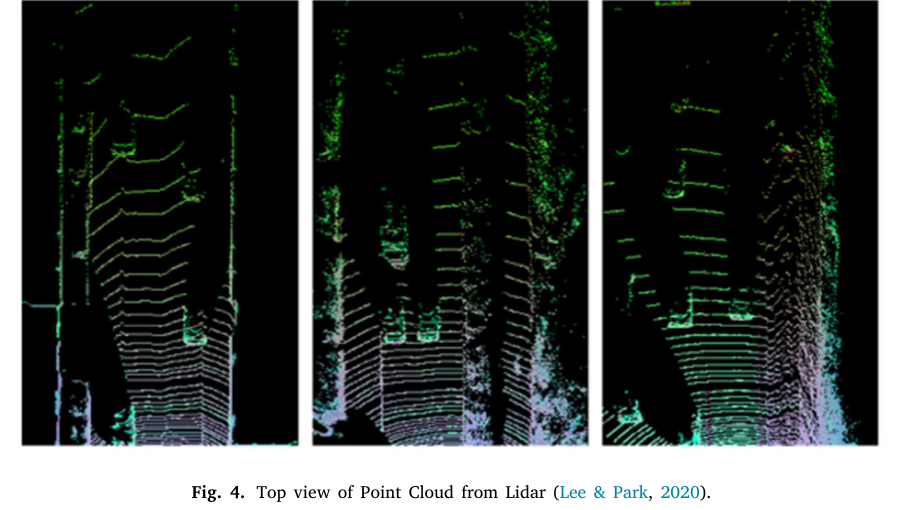
\includegraphics[width=0.5\textwidth]{img/12Screenshot_20231106_142954}\label{fig:12}
    \end{subfigure}
    \begin{subfigure}
        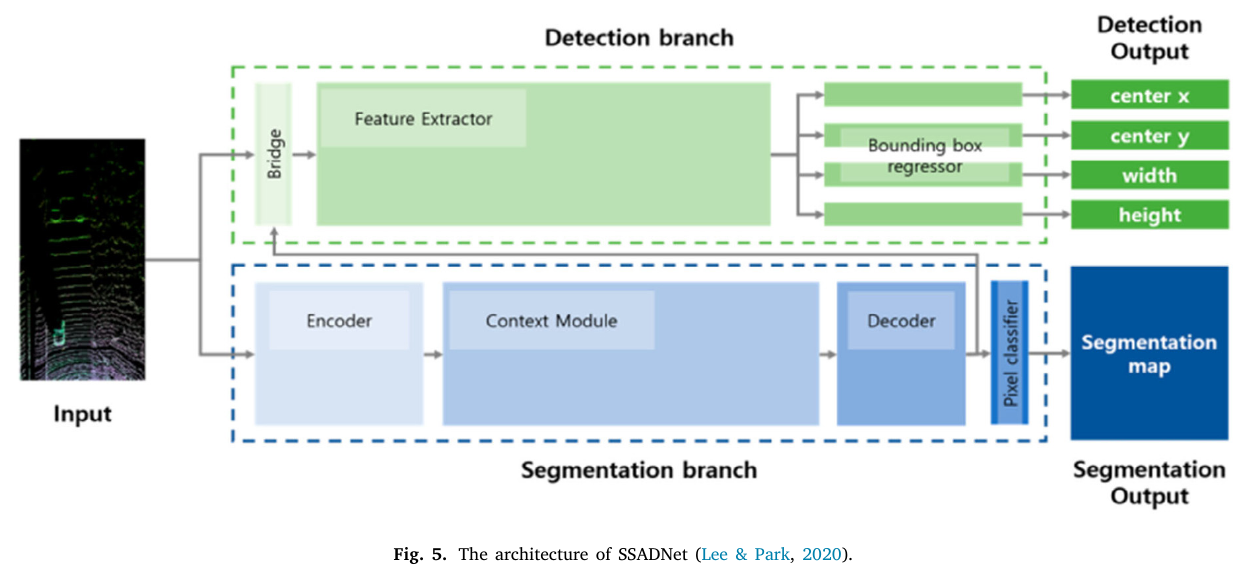
\includegraphics[width=0.5\textwidth]{img/13Screenshot_20231106_143018}\label{fig:13}
    \end{subfigure}
    \begin{subfigure}
        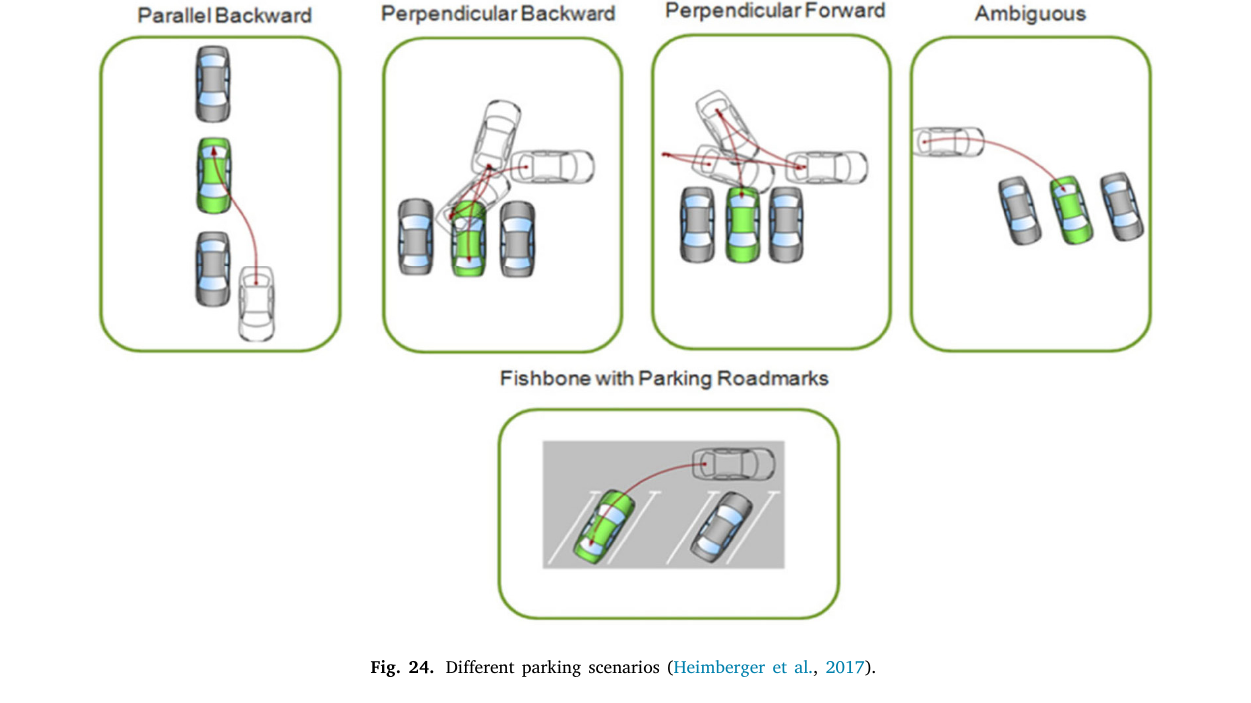
\includegraphics[width=0.5\textwidth]{img/15Screenshot_20231106_143633}\label{fig:15}
    \end{subfigure}
    \begin{subfigure}
        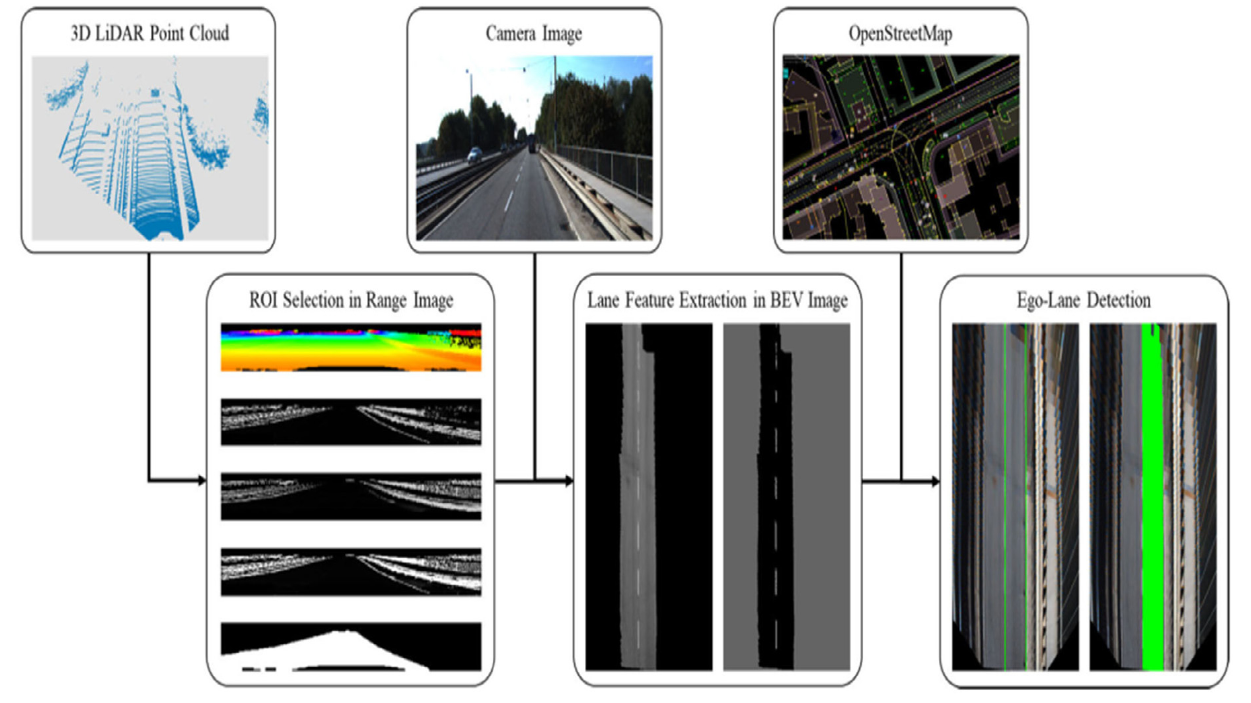
\includegraphics[width=0.5\textwidth]{img/14 Screenshot_20231106_143419}\label{fig:14}
    \end{subfigure}
    \begin{subfigure}
        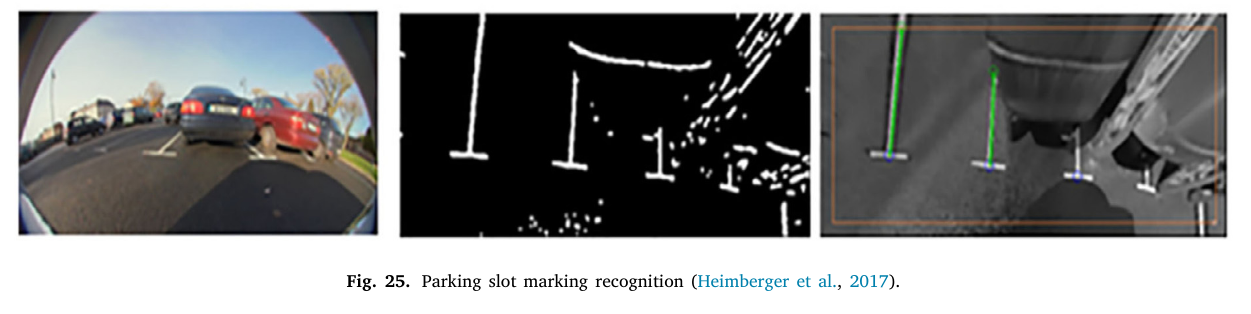
\includegraphics[width=0.99\textwidth]{img/16Screenshot_20231106_143701}\label{fig:16}
    \end{subfigure}
\end{figure}
\clearpage

\subsection{
    \textbf{Vision-based autonomous car racing using deep imitative reinforcement learning}
    ~\cite{cai2021vision}
}\label{subsec:vision-based-autonomous-car-racing}
El artículo fue publicado en la revista IEEE Robotics and Automation Letters en 2021 y aborda el desafío del automovilismo autónomo
en el campo del control robótico, históricamente dependiente de mapas precisos, localización y planificación, lo que lo hace
computacionalmente ineficiente y sensible a cambios en el entorno.
\\
Se destaca el desarrollo de sistemas de aprendizaje profundo de extremo a extremo, que muestran resultados prometedores en la conducción
autónoma.
\\
Sin embargo, estos sistemas suelen basarse en aprendizaje por imitación supervisada (IL), enfrentando problemas de discrepancia
en la distribución de datos.
\\
Aunque se han empleado métodos de aprendizaje por refuerzo (RL), requieren grandes cantidades de datos de interacción riesgosa.
\\
El artículo presenta un enfoque innovador denominado aprendizaje profundo imitativo y de refuerzo (DIRL), que logra la agilidad en
el automovilismo autónomo mediante el uso de entradas visuales.
\\
Este enfoque combina el conocimiento adquirido tanto del aprendizaje por imitación como del aprendizaje basado en modelos de RL,
permitiendo al agente aprender de instructores humanos y mejorar su rendimiento interactuando con un modelo de mundo offline.
La validación del algoritmo se lleva a cabo tanto en simulaciones de conducción de alta fidelidad como en un automóvil RC a escala 1/20 en
el mundo real, con capacidad computacional limitada. \\
Los resultados de la evaluación demuestran que este método supera a enfoques anteriores de IL y RL en eficiencia de muestra y rendimiento
en la tarea, mostrando un gran potencial en el ámbito de la conducción autónoma.
\begin{figure}[!ht]
    \begin{subfigure}
        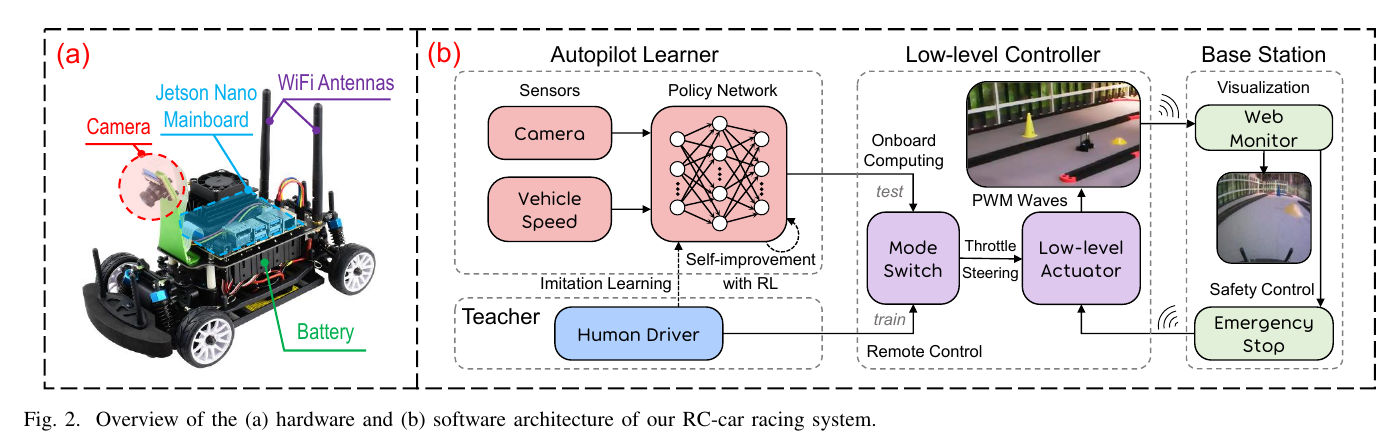
\includegraphics[width=\textwidth]{img/21}\label{fig:21}
    \end{subfigure}
    \begin{subfigure}
        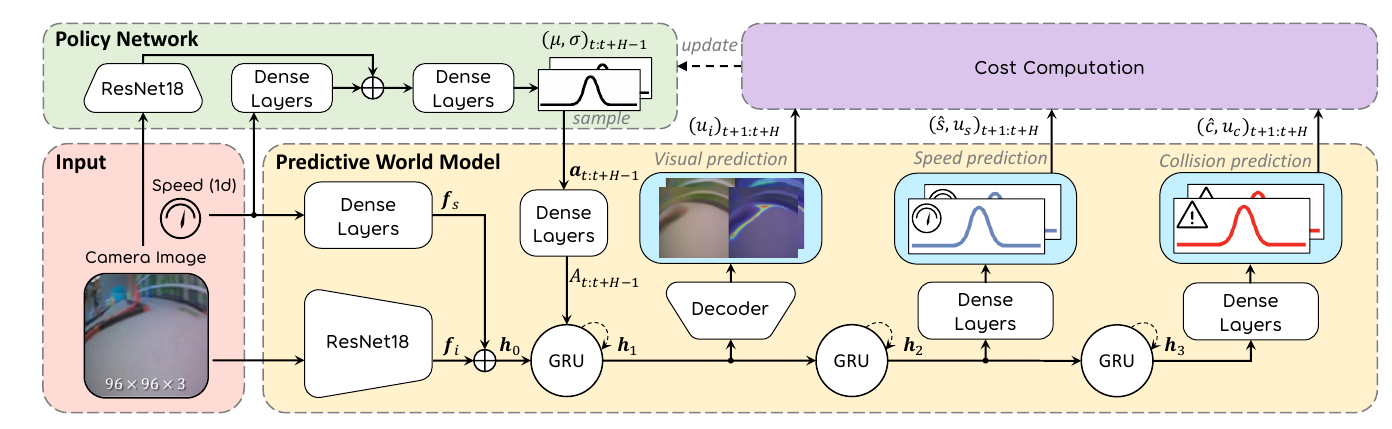
\includegraphics[width=\textwidth]{img/22}\label{fig:22}
    \end{subfigure}
%            \begin{subfigure}
%                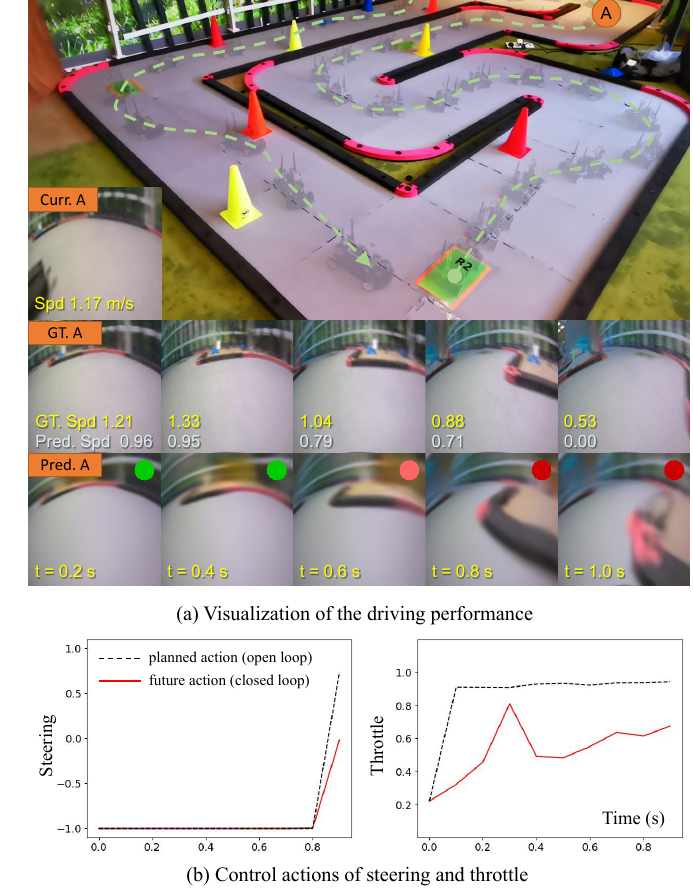
\includegraphics[width=0.2\textwidth]{img/23}\label{fig:23}
%            \end{subfigure}
\end{figure}

\clearpage

\subsection{
    \textbf{Model-based probabilistic collision detection in autonomous driving}
    ~\cite{althoff2009model}
}\label{subsec:probabilistic-collision-detection}
El artículo fue publicado en la revista IEEE Transactions on Intelligent Transportation Systems en 2009 y se centra en la seguridad vial
de los vehículos autónomos en entornos de tráfico complejo.
Su enfoque principal es la detección probabilística de colisiones mediante el análisis y la predicción de la ocupación de la carretera
por parte de otros vehículos.\\
El estudio aborda la incertidumbre inherente en la interacción entre los vehículos autónomos y otros actores del tráfico.
Analiza cómo las mediciones y los posibles comportamientos de estos afectan la predicción de posibles colisiones.
Además, considera las limitaciones en las maniobras de conducción debidas a la geometría de la carretera y la influencia
de estas restricciones en la probabilidad de colisión para trayectorias específicas.\\
Lo más destacado de este enfoque es su eficiencia. La mayor parte de los cálculos intensivos se llevan a cabo offline,
permitiendo disponer de un algoritmo en línea eficiente para aplicaciones en tiempo real.                                                                           \\
Esto contribuye significativamente a la seguridad vial al proporcionar una herramienta precisa y eficaz para la detección anticipada de
posibles colisiones en entornos de conducción autónoma.                                                            \\
\begin{figure}[!ht]
    \begin{subfigure}
        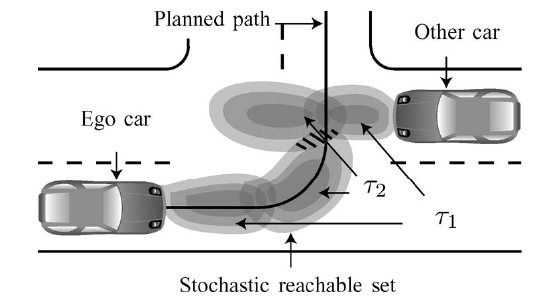
\includegraphics[width=0.5\textwidth]{img/31}\label{fig:31}
    \end{subfigure}
    \begin{subfigure}
        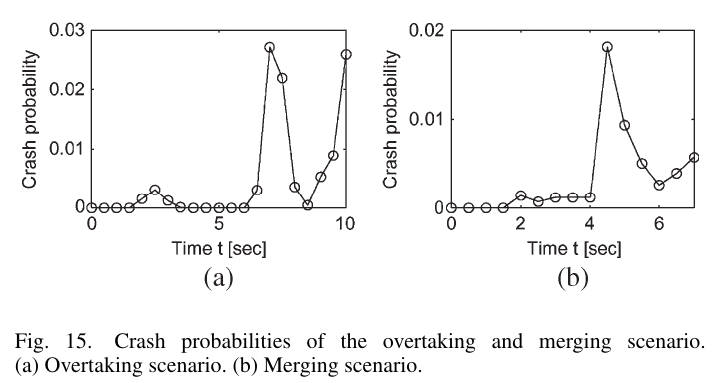
\includegraphics[width=0.5\textwidth]{img/35}\label{fig:35}
    \end{subfigure}
%            \begin{subfigure}
%                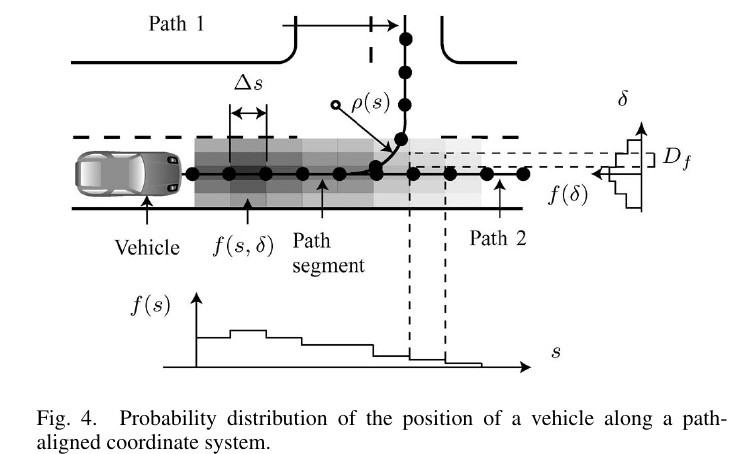
\includegraphics[width=0.5\textwidth]{img/32}\label{fig:32}
%            \end{subfigure}
    \vspace{2cm}
    \begin{subfigure}
        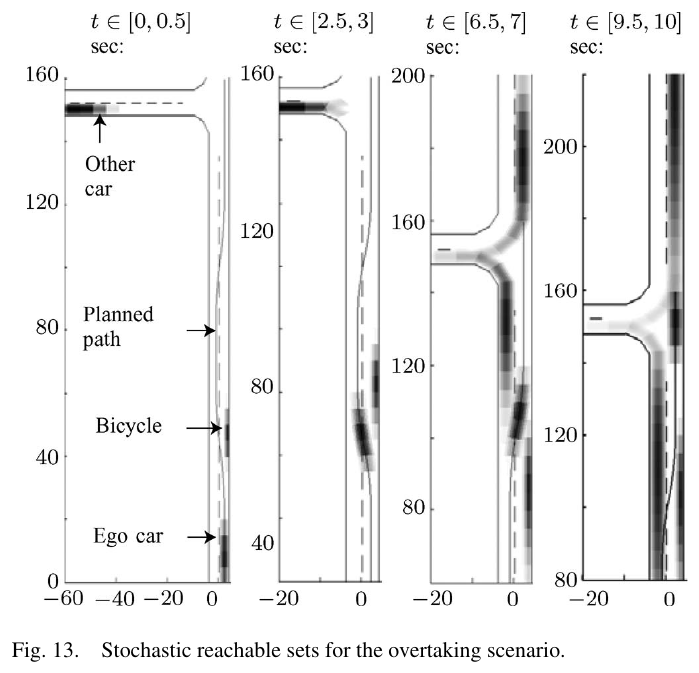
\includegraphics[width=0.5\textwidth]{img/33}\label{fig:33}
    \end{subfigure}
    \begin{subfigure}
        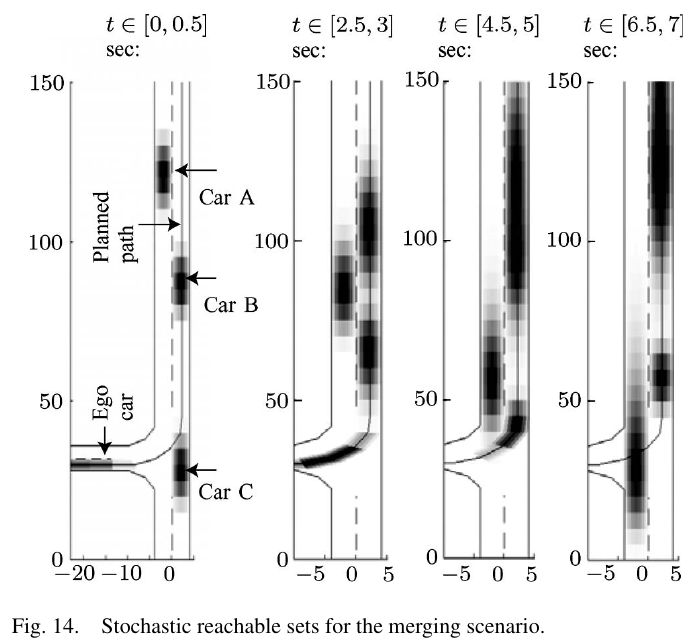
\includegraphics[width=0.5\textwidth]{img/34}\label{fig:34}
    \end{subfigure}

\end{figure}
\clearpage

\subsection{
    \textbf{Vision-based autonomous vehicle systems based on deep learning: A systematic literature review}
    ~\cite{pavel2022vision}
}\label{subsec:vision-based-autonomous-vehicle}
El artículo fue publicado en la revista Applied Science en 2022 y presenta una revisión sistemática de la literatura sobre el empleo
de técnicas de aprendizaje profundo en los sistemas
de vehículos autónomos a lo largo de la última década.                                                                    \\Esta revisión se divide en varios módulos que abarcan distintos aspectos,
desde el análisis de percepción y la toma de decisiones hasta el control, la planificación de trayectorias
y la visualización en sistemas de realidad aumentada tipo HUD.                                                                                                                   \\
Se examinan investigaciones llevadas a cabo entre 2011 y 2021 que se enfocan en la utilización de cámaras RGB como sensores principales
en estos sistemas. Se otorga especial atención a los resultados finales, destacando la visualización en sistemas de realidad aumentada
basados en HUD.                                                                                                      \\Esto incluye advertencias tempranas, marcadores en la carretera para mejorar la navegación y la seguridad, superposición
de información en vehículos y peatones en condiciones visuales extremas para reducir colisiones.
La revisión subraya los métodos actuales de aprendizaje profundo que se basan únicamente en la visión de cámaras RGB, prescindiendo de la
compleja fusión de sensores.                                                                     \\Se espera que este enfoque allane el camino para el desarrollo ágil de sistemas de vehículos autónomos,
siendo prácticos, eficientes y seguros en términos de costos.                                                               \\
\begin{figure}[!ht]
    \begin{subfigure}
        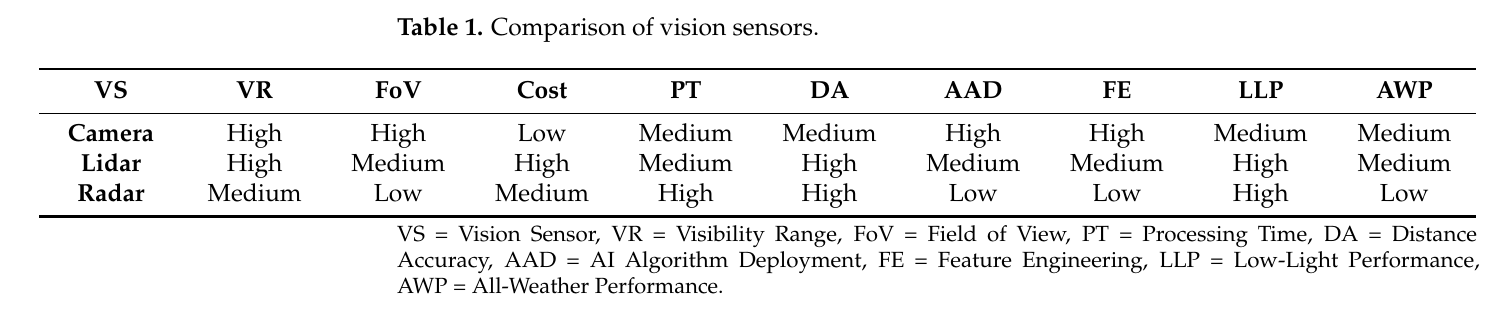
\includegraphics[width=1\textwidth]{img/71}\label{fig:71}
    \end{subfigure}
%            \begin{subfigure}
%                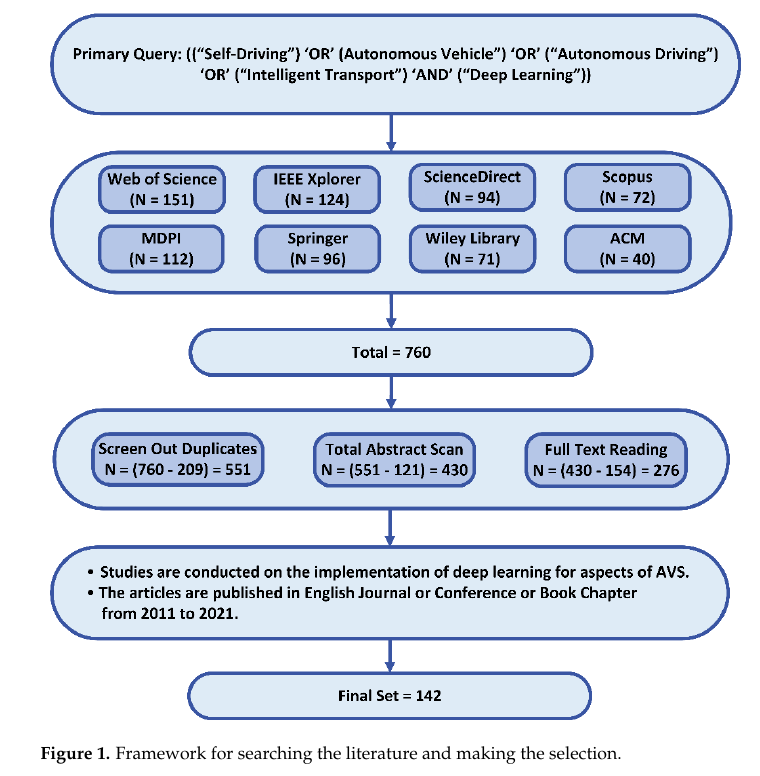
\includegraphics[width=0.5\textwidth]{img/72}\label{fig:72}
%            \end{subfigure}
    \begin{subfigure}
        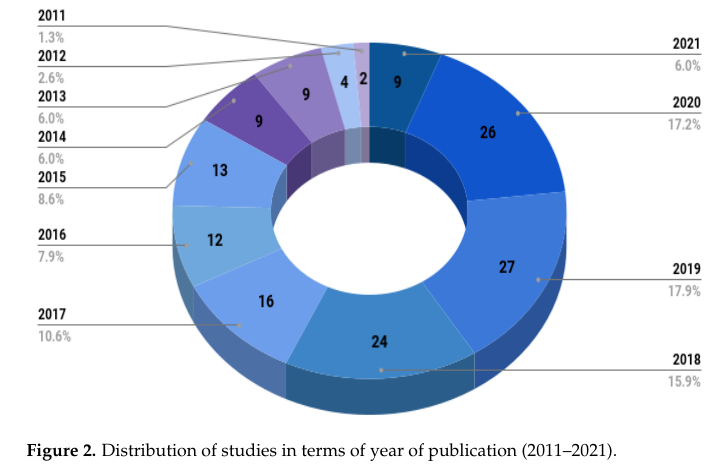
\includegraphics[width=0.5\textwidth]{img/73}\label{fig:73}
    \end{subfigure}
    \begin{subfigure}
        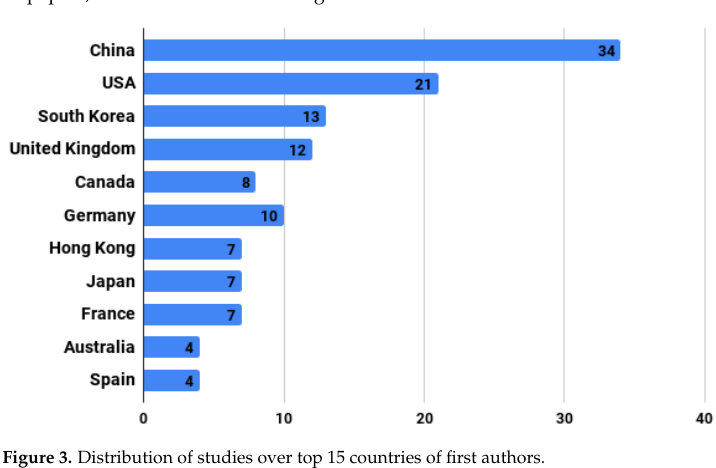
\includegraphics[width=0.5\textwidth]{img/74}\label{fig:74}
    \end{subfigure}
\end{figure}
\clearpage

\subsection{
    \textbf{A cost-effective computer vision-based vehicle detection system}
    ~\cite{alam2022cost}
}\label{subsec:cost-effective-vehicle-detection}
El artículo fue publicado en la revista Concurrent Engineering en 2022 y se enfoca en la detección de vehículos.
\\Destaca la importancia crítica del procesamiento rápido y la detección precisa de vehículos dentro de un sistema autónomo de detección.
\\Presenta un sistema de detección de vehículos basado en visión por computadora que utiliza un algoritmo de Gentle Adaptive Boosting
con características tipo Haar para generar hipótesis de vehículos de manera eficiente.
Para abordar los errores potenciales, propone el uso de un algoritmo de Máquinas de Vectores de Soporte (SVM) entrenado con características
del histograma de gradientes orientados (HOG) para filtrar las hipótesis falsas.
\\El descriptor HOG se centra en la forma y contornos de los vehículos, mejorando la precisión de la detección.
La combinación de características tipo Haar y HOG permite cumplir los objetivos de detección en la conducción autónoma.
\\El rendimiento del sistema propuesto se evalúa con imágenes capturadas durante el día y la noche y se compara con tres detectores
de vehículos existentes. Los resultados muestran una precisión promedio del 0.97 para imágenes capturadas durante el día
y del 0.94 para imágenes nocturnas.                                                                                               \\Además, se destaca que el sistema propuesto requiere aproximadamente 15 veces menos tiempo
de entrenamiento en comparación con las técnicas existentes, utilizando la misma cantidad de datos de imágenes y la misma unidad
de procesamiento central (CPU). Esto demuestra una mejora significativa en la eficiencia del sistema propuesto en términos de tiempo de entrenamiento.
\begin{figure}[!ht]
%            \begin{subfigure}
%                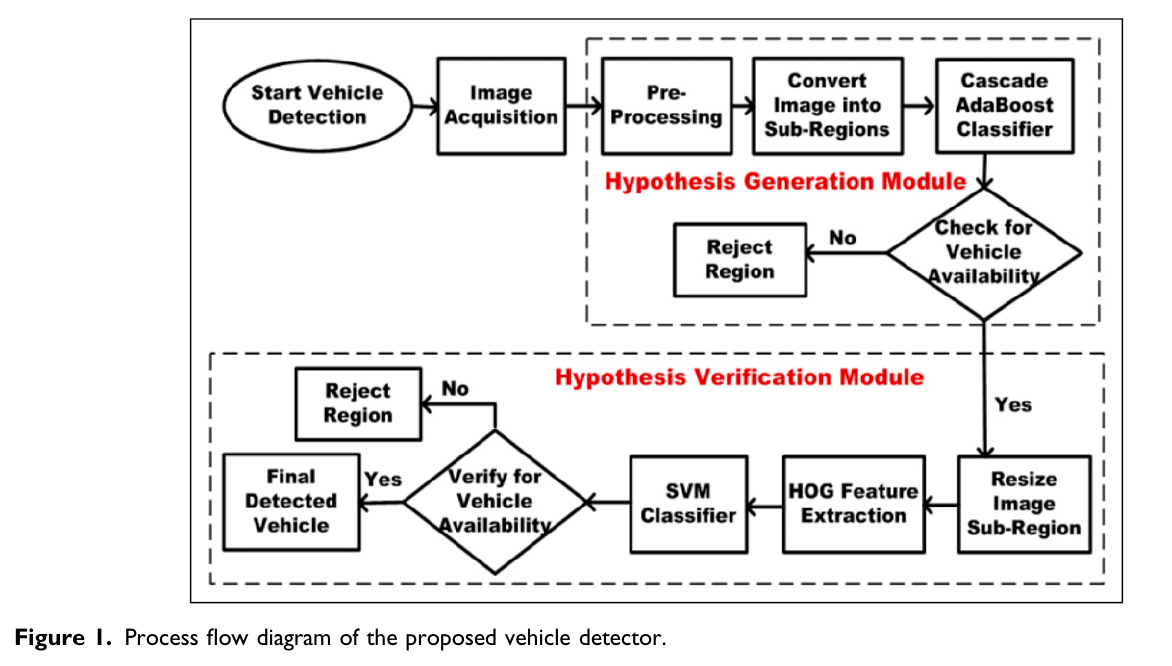
\includegraphics[width=0.6\textwidth]{img/81}\label{fig:81}
%            \end{subfigure}
%            \begin{subfigure}
%                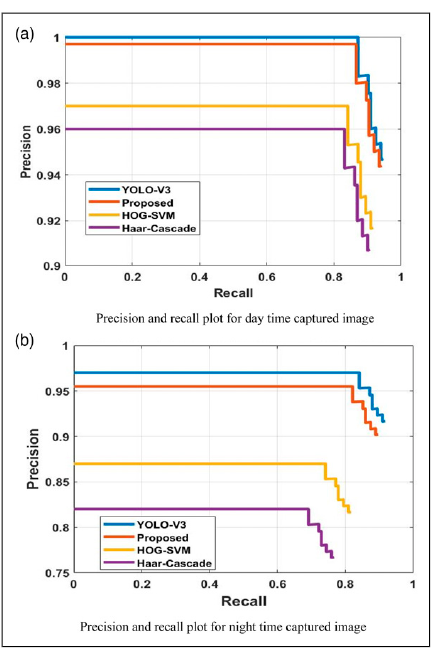
\includegraphics[width=0.5\textwidth]{img/86}\label{fig:82}
%            \end{subfigure}
    \begin{subfigure}
        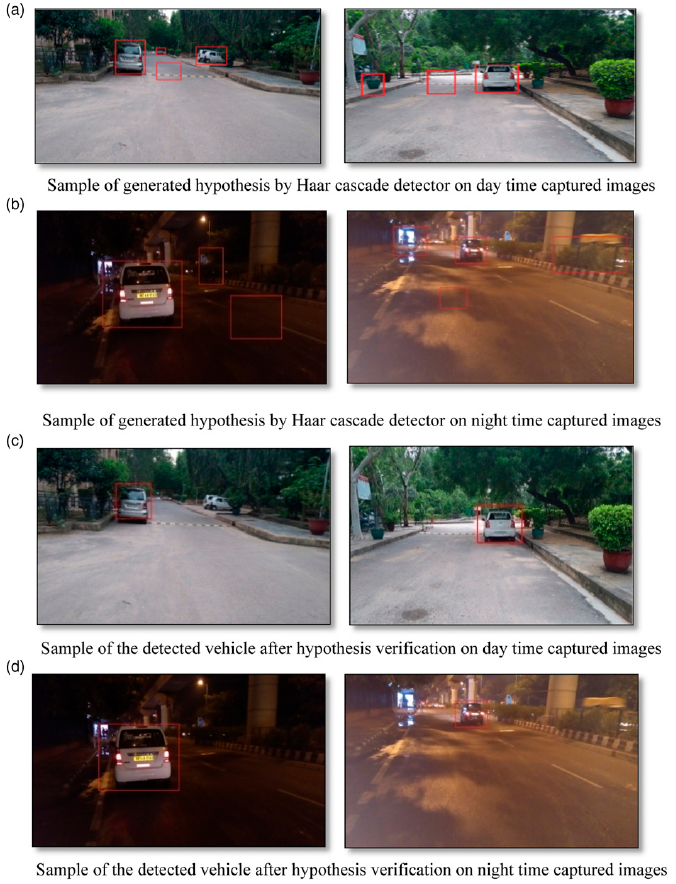
\includegraphics[width=0.5\textwidth]{img/84}\label{fig:84}
    \end{subfigure}
    \begin{subfigure}
        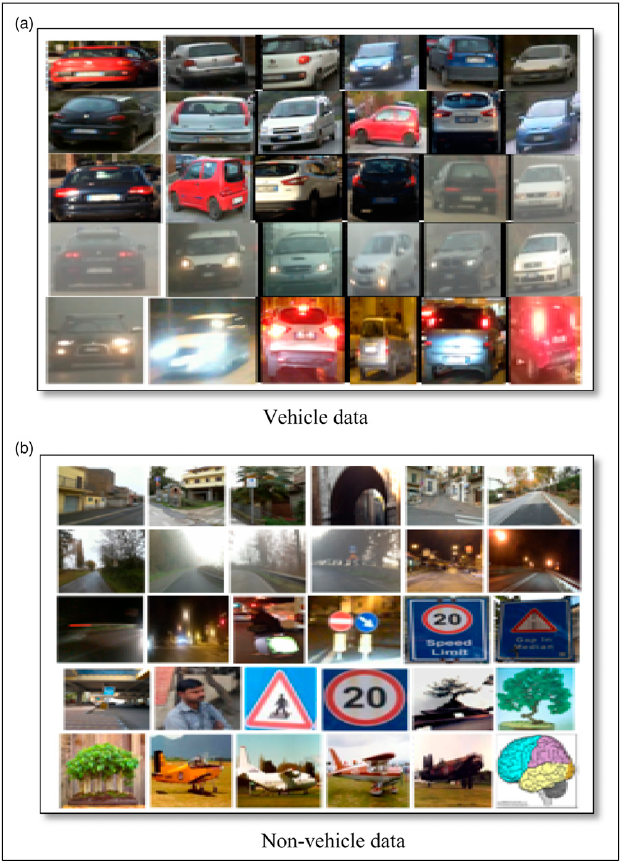
\includegraphics[width=0.5\textwidth]{img/82}\label{fig:86}
    \end{subfigure}
\end{figure}
\clearpage


    \section*{Tabla comparativa}
    \begin{center}
        \resizebox{\textwidth}{!}{
            \begin{tabular}{|p{5cm}|p{2cm}|p{2cm}|p{2cm}|p{2cm}|p{2cm}|p{2cm}|}
                \hline
                \textbf{Características}
                & \textbf{Propia}
                & \textbf{Autonomous Driving Architectures \cite{bachute2021autonomous}}
                & \textbf{Vision-based Autonomous Car Racing \cite{cai2021vision}}
                & \textbf{Model-based Probabilistic Collision Detection \cite{althoff2009model}}
                & \textbf{Vision-based Autonomous Vehicle Systems \cite{pavel2022vision}}
                & \textbf{Cost-effective Vehicle Detection System \cite{alam2022cost}} \\
                \hline
                Uso de algoritmos de Aprendizaje Automático y Aprendizaje Profundo & X & X &   &   & X &   \\
                \hline
                Enfoque en la conducción autónoma                                  & X & X & X & X & X & X \\
                \hline
                Ventajas de la conducción autónoma                                 & X & X &   &   &   &   \\
                \hline
                Complejidad de los sistemas de conducción autónoma                 &   & X &   &   &   &   \\
                \hline
                Análisis de tareas en la conducción autónoma                       & X & X &   &   &   &   \\
                \hline
                Evaluación y comparación de algoritmos                             &   & X & X &   &   &   \\
                \hline
                Predicción estocástica de ocupación de la carretera                &   &   &   & X &   &   \\
                \hline
                Eficiencia en cálculos intensivos                                  &   &   & X & X &   &   \\
                \hline
                Utilización de cámaras RGB como sensores principales               & X &   & X &   & X &   \\
                \hline
                Detección de vehículos en conducción autónoma                      & X &   &   &   &   & X \\
                \hline
            \end{tabular}
        }
    \end{center}
    \clearpage

    \section*{Metodología}
    \justify
    La metodología propuesta se fundamenta en un enfoque iterativo que abarca diversas etapas para la implementación del sistema
    de estimación de la posición relativa al estacionamiento de un vehículo mediante cámaras y sensores para parqueo automático en simulación.
    En primera instancia, se establecerá un entorno de simulación realista que refleje el escenario de un vehículo en movimiento y su entorno de estacionamiento.
    Posteriormente, se procederá a la adquisición y procesamiento de datos provenientes de los sensores de dicho entorno simulado.
    La fase siguiente implicará el diseño y la implementación de algoritmos de visión computacional para la detección temprana de eventos críticos en tiempo real.
    Estos algoritmos serán sometidos a un proceso de entrenamiento y ajuste utilizando técnicas de aprendizaje automático.
    Finalmente, se llevarán a cabo pruebas exhaustivas y evaluaciones para validar la efectividad y la precisión del sistema propuesto en situaciones simuladas.

    \section*{Calendario de actividades}
    \begin{center}
        \resizebox{\textwidth}{!}{
            \begin{tabular}{|p{3cm}|*{17}{p{1cm}|}}
                \hline
                \textbf{Actividad} & \multicolumn{17}{c|}{\textbf{Duración}} \\
                \hline
                & Ene & Feb & Mar & Abr & May & Jun & Jul & Ago & Sep & Oct & Nov & Dic
                & Ene & Feb & Mar & Abr & May \\
                \hline
                Investigación y revisión bibliográfica      & \cellcolor{gray!30} & \cellcolor{gray!30} & & & & & & & & & & & & & & & & \\
                \hline
                Diseño y Configuración del Entorno Simulado &                     & \cellcolor{gray!30} & \cellcolor{gray!30} & \cellcolor{gray!30} & & & & & & & & & & & & & & \\
                \hline
                Adquisición y Procesamiento de Datos        &                     &                     &                     &                     & \cellcolor{gray!30} & \cellcolor{gray!30} & \cellcolor{gray!30} & & & & & & & & & & & \\
                \hline
                Desarrollo y Entrenamiento de Algoritmos    &                     &                     &                     &                     &                     &                     & \cellcolor{gray!30} & \cellcolor{gray!30} & \cellcolor{gray!30} &  & & & & & & & & \\
                \hline
                Evaluación y Ajuste del Sistema             &                     &                     &                     &                     &                     &                     &                     & \cellcolor{gray!30} & \cellcolor{gray!30} & \cellcolor{gray!30} & \cellcolor{gray!30} & & & & & & & \\
                \hline
                Documentación y Análisis de Resultados      &                     &                     &                     &                     &                     &                     &                     &                     & \cellcolor{gray!30} & \cellcolor{gray!30} & \cellcolor{gray!30} & \cellcolor{gray!30} & \cellcolor{gray!30} & & & & & \\
                \hline
                Redacción y Revisión del documento de tesis &                     &                     &                     &                     &                     &                     &                     &                     &                     &                     & \cellcolor{gray!30} & \cellcolor{gray!30} & \cellcolor{gray!30} & \cellcolor{gray!30} & \cellcolor{gray!30} & \cellcolor{gray!30} & \cellcolor{gray!30} & \\
                \hline
            \end{tabular}
        }
    \end{center}
    \clearpage

    \section*{Referencias bibliográficas}
    \bibliographystyle{acm}
    \bibliography{referecias}
\end{document}
